
%----------------------------------------------------------------------------------------
%	PART
%----------------------------------------------------------------------------------------


\part{Capítulo cuatro}

\graphicspath{ {img/ch4/}, {img/} }

%----------------------------------------------------------------------------------------
%	CHAPTER 4
%----------------------------------------------------------------------------------------

\chapterimage{ima2} % Chapter heading image


\chapter{Serie uniforme vencida y anticipada}



\section{{Fórmulas del capítulo}}

\begin{spacing}{1.2}
\begin{center}
\begin{tabular}{ |p{4.2cm}|p{5.7cm}| p{4cm}|}
\hline 
\rowcolor{orange!50}              %
\begin{center}\textbf{Fórmula} \end{center} & \begin{center} \textbf{Nombre}\end{center} & \begin{center} \textbf{Excel} \end{center} \\ \hline                        


$VP = R  \frac{1-(1 + i)^{-n}}{i} $\hspace{35 pt} & Valor presente serie uniforme vencida & VNA(i;R1;R2;R3;...)\\ \hline 


	 $VF = R  \frac{(1 + i)^n-1}{i} $ &  Valor futuro serie uniforme vencida \hspace{35 pt} & VF(i;n;;VA,0)\\  \hline 


$VP_{a} = R  \frac{1-(1 + i)^{-n}}{i}  (1 + i) $ \hspace{35 pt} & Valor presente serie uniforme anticipada   & - \\ \hline 

$VF_{a} = R  \frac{(1 + i)^n-1}{i}   (1 + i) $ \hspace{35 pt} &  Valor futuro serie uniforme anticipada  & VF(i;n;;VA,1) \\ \hline 


 
\end{tabular}
\end{center}
\end{spacing}

\textbf{Ejemplo 1}\\

Una persona compra un terreno cuyo valor al contado es de \$2 millones. Si le dan la facilidad para pagarlo en cuatro cuotas iguales trimestrales de R c/u, que se efectuarán al final de cada trimestre y, además se le cargaría un interés del 40\% nominal anual trimestre vencido, hallar el valor de la cuota trimestral de amortización.\\\\
\textbf{Solución:}\\\\
Primero se construye un diagrama que muestre las fechas, el valor de la deuda y el valor de los pagos (flujo de caja). Puesto que la tasa es nominal anual  trimestre vencido y los pagos son  periódicos trimestrales se usará el trimestre como período.	
Planteando la ecuación de valor con fecha focal al comienzo quedaría así:

\clearpage

a. Diagrama de Flujo: \\
El diagrama representa una salida de dinero de \$2'000.000 de contado o 4 cuotas periodicas con intereses para pagar los mismos \$2'000.000. Con fecha de pago al día de hoy.

\begin{center}
	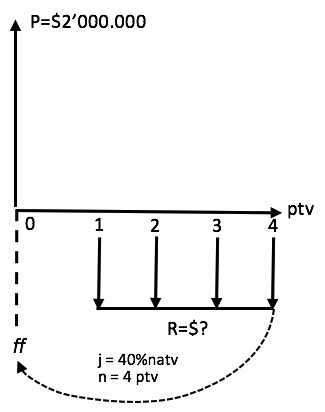
\includegraphics[height=6cm]{4_1}
\end{center}

b. Declaración de variables\\ \\


	
	    $P=\$2'000.000$\\
	$	R=\$?$
		\\
		j=40 \% natv
		\\
		i=$\frac{40}{4}=10\%$ ptv\\
		$n_{1}=1 ptv$\\
		$n_{2}=2 ptv$\\
		$n_{3}=3 ptv$\\
		$n_{4}=4 ptv$\\
		


c. Declaración de fórmulas \\



	%	VF=P(1+i)^{n}\ \ Valor \ \ futuro
	%	\\
	P=F(1+i)^{-n} \hspace{35} \textit{Valor Presente} \\
	


d. Desarrollo matemático \\



Se plantea la ecuación de valor colocando la fecha focal en cero, quedando así al reemplazar los valores:\\

	$P=R(1+i)^{-n_1 }+R(1+i)^{-n_2 }+R(1+i)^{-n_3}+R(1+i)^{-n_4}$ \hspace{8} \textit{Ecuación de valor}\\

$	\$2.000.000=R(1+0.1)^{-1}+R(1+0.1)^{-2}+R(1+0.1)^{-3 }+R(1+0.1)^{-4}$ \\


Factorizando R se tendrá:\\


		\$2.000.000=R[(1.1)^{-1}+(1.1)^{-2}+(1.1)^{-3 }+(1.1)^{-4 }]
		\\
		\$2.000.000=R(3,169865)
		\\
		R=\$630.941,61\\    

e. Respuesta \\



El valor de la cuota de la serie uniforme es de \$630.941,61 \\

\textbf{Planteando la ecuación de valor con fecha focal al final quedaría así:      }
\\\\
{a.  Diagrama de Flujo:} \\
El diagrama representa el valor del pago de contado del terreno equivalente a \$2.000.000 de contado, y cuotas periódicas con intereses para pagar los mismos \$2.000.000. Con fecha de pago al día al final de los cuatro períodos trimestrales.

\begin{center}
	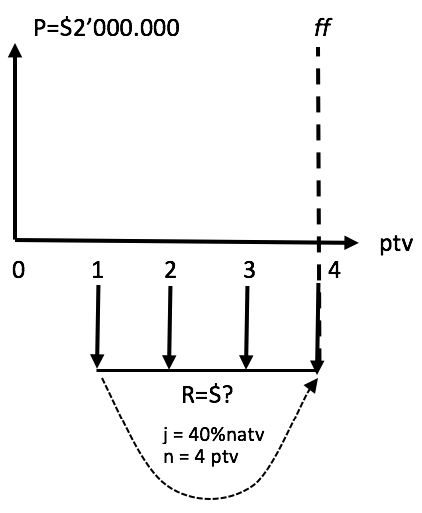
\includegraphics[height=6cm]{4_2}
\end{center}

b. Declaración de variables \\

        P= \$2.000.000\\
        $i=10\%$ \ ptv\\        
		$n_{1}=1$ ptv
		\\
		$n_{2}=2$ ptv
		\\
		$n_{3}=3$ ptv
		\\
		$n_{4}=4$ ptv
		\\
	


c. Declaración de fórmulas\\

		F=P(1+i)^{n} \hspace{35} \textit{Valor Futuro} \\


d. Desarrollo matemático \\

	$	\$2.000.000(1+ 0.1)^{4}=R(1+ 0.1)^{0}+R(1+ 0.1)^{1}+R(1+ 0.1)^{2 }+R(1+ 0.1)^{3}$ \hspace{8} \textit{Ecuación de valor}\\


Factorizando se tiene:\\

	$	\$2.000.000(1.1)^{4}=R[(1.1)^{0}+(1.1)^{1}+(1.1)^{2 }+(1.1)^{3} 
		\\
		\$2.928.200=R(4,641)
		\\
		R=\$630.941,61\\$
		\\
		\\
e. Respuesta: \\

El valor de la cuota trimestral es de \$630.941,61 tomando como fecha focas el final del flujo, valor equivalente si se toma al inicio.
\\

Se observa a primera vista que la ecuación tiene una presentación muy distinta pero el resultado final es el mismo. El problema anterior no presentó dificultad para resolverlo; pero, si el número de pagos hubiese aumentado considerablemente, la solución no hubiese sido tan sencilla, como en el caso de pagar una deuda mediante pagos mensuales, durante 20 años. 
La solución de este problema ha dado origen a un modelo matemático llamado serie uniforme. Antes de entrar a estudiar las series periódicas se darán algunas definiciones.

\subsection{Ingresos:}Es la renta recibida en forma periódica de igual valor que corresponde a la cuota del ejemplo anterior. A la renta también se le conoce como cuota.

\subsection{Período:}
Es el intervalo de tiempo de una serie uniforme.

\subsection{Serie uniforme:}
Una serie uniforme es una serie de pagos o ingresos que cumple con las siguientes condiciones:


\hspace{35}	1. Todos los pagos o ingresos (según sea el caso) son de igual valor.

\hspace{35} 2. Todos los pagos o ingresos (según sea el caso) se hacen a iguales intervalos de tiempo.

\hspace{35} 3. A todos los pagos o ingresos (según sea el caso) se les aplica la misma tasa de interés.

\hspace{35}	4. El número de pagos o ingresos (según sea el caso) es igual al número de períodos.


La \textbf{primera condición} es indispensable para poder factorizar tal como se hizo cuando se plantearon las ecuaciones de valor del ejemplo 1.
\\\\
La \textbf{segunda condición} establece que los pagos o ingresos deben hacerse a iguales intervalos de tiempo, esto es necesario para que los exponentes sean ascendentes o descendentes tal como se ve en las ecuaciones del ejemplo anterior. Esta condición se cumple aún si los pagos o ingresos son trimestrales, semestrales o anuales y sin embargo a la serie se le sigue denominando serie uniforme.
\\\\
La \textbf{tercera condición} establece que todos los pagos o ingresos deben ser llevados a valor presente o a valor final, según el caso, a la misma tasa de interés. Esto nos garantiza que todos los términos dentro del paréntesis angular tienen la misma base, por lo tanto, la serie que está dentro del paréntesis angular forma una progresión geométrica.
\\\\
La \textbf{cuarta condición} establece que el número de pagos o ingresos debe ser igual al número de períodos.
\\\\
Por tanto la serie que se muestra en la siguiente gráfica no representa una serie uniforme porque \textbf{tiene 3 pagos y solo hay 2 períodos}

\begin{center}
	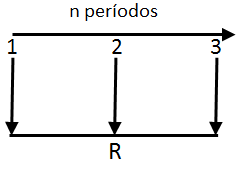
\includegraphics[height=3cm]{4_3}
\end{center}

Para que la gráfica anterior represente una serie uniforme bien conformada es necesario agregarla un período que bien puede quedar al principio o al final. En el primer caso se tendrá:

\begin{center}
	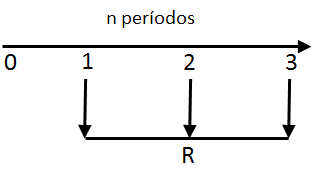
\includegraphics[height=2.5 cm]{4_4}
\end{center}

La serie uniforme así conformada recibe el nombre de serie uniforme ordinaria o \textbf{serie uniforme vencida} que viene a ser aquella en que los pagos se efectúan al final del período por ejemplo el pago de los sueldos de un empleado (primero viene el período de trabajo y después viene el pago) 
\\\\
En el segundo caso se tendrá:

\begin{center}
	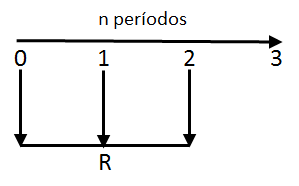
\includegraphics[height=2.7 cm]{4_5}
\end{center}

La serie uniforme así conformada recibe el nombre de \textbf{serie uniforme anticipada} porque los pagos se efectúan al principio del período, por ejemplo el pago mensual del arriendo de una casa (primero paga y después tiene derecho a ocupar la casa durante el mes que pagó). 
\\\\
La siguiente gráfica no representa una serie uniforme porque hay 3 pagos y hay 4 períodos.

\begin{center}
	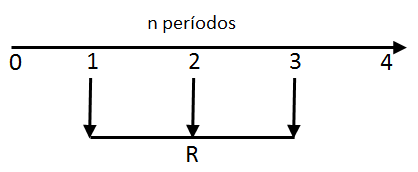
\includegraphics[height=2.7cm]{4_6}
\end{center}

Claramente puede observarse que cuando se inicia la gráfica con pago y se termina con pago, como ocurre en la gráfica 1, no hay una serie uniforme bien conformada y cuando la gráfica inicia con período y termina con período, como en el caso de la gráfica 4, tampoco hay una serie uniforme bien conformada. Las gráficas 2 y 3 si representan series periódicas bien conformadas y tienen una característica en común, que su inicio y fin son diferentes, en la gráfica 2 se inicia con período y se termina con pago y en la gráfica 3 se inicia con pago y se termina con período.
\\\\
En conclusión para que una serie uniforme éste bien conformada su \textbf{inicio y fin deben ser diferentes.}

\section{Plazo de una serie uniforme}
El tiempo que transcurre entre el inicio del primer período y el final del último período se denomina período de la serie uniforme (mensual, trimestral, semestral, etc.)  y se representa por n.
Una serie uniforme tiene dos valores, el valor final y el valor presente, en el primer caso todos los pagos son trasladados al final de la serie uniforme y en el segundo caso todos los pagos son trasladados al principio de la serie uniforme

\section{Valor futuro (VF, R, i, n)}
El valor futuro se representa como VF
\\\\
En forma general se tendrá:

\begin{center}
	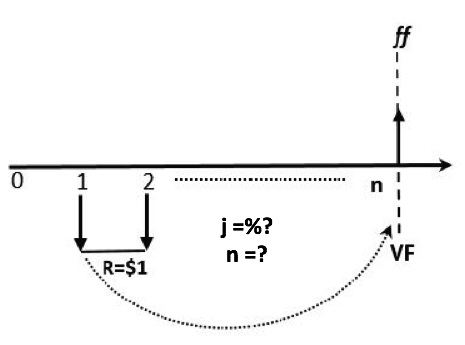
\includegraphics[height=6cm]{4_7}
\end{center}

Para plantear la ecuación de valor con fecha focal en \textbf n \textbf trasladamos cada uno de los pagos de \$1  a valor final usando la ecuación del interés  compuesto.\\


	VF= VP (1+i)^{n} \hspace{35} \textit{Valor Futuro} \\


A cada pago, pero en cada caso, P=1. El pago que está en 1 se traslada por \textbf n-1 \textbf períodos y el que está en 2 se traslada por \textbf n-2  \textbf períodos y así sucesivamente hasta llegar al pago que está en \textbf n \textbf el cual no se traslada por estar  en la fecha focal entonces:

\begin{equation*}
	VF=1+ (1+i) +(1+i)^{2}+....+(1+i)^{n-1}  \ \ [1]
\end{equation*}

Si la ecuación (1) la multiplicamos por (1+i) obtenemos la ecuación (2) entonces:\\


	VF(1+i)= (1+i) +(1+i)^{2}+....+(1+i)^{-n} \ \ [2]\\

Substrayendo la ecuación (1) de la ecuación (2), tenemos la ecuación (3):\\

%begin{equation*}
%	\begin{split}
		$VF(1+i)= (1+i)+(1+i)^{2}+...+(1+i)^{-n}$
		\\
		$VF=1+(1+i)+(1+i)^{2}+...+(1+i)^{n-1}$ \\ 
		$VF (1+i) - VF = ((1+i)^{n}) -1$ \ \ [3]\\
%	\end{split}
%\end{equation*}

Factorizando VF se tiene la ecuación (4)\\

%\begin{equation*}
	$F(i)=(1+i)^{n-1}$ \ \ [4]\\ \\
%\end{equation*}
Finalmente despejando VF se tiene la ecuación (5)\\
%\begin{equation*}
\\
	$VF = \frac {R((1+i)^n-1)}{i}$ \ \ [5] \hspace{35} \textit{Valor futuro de una serie uniforme vencida} \\
%\end{equation*}

\section{Valor presente (VP, R, i, n)}

El caso del valor presente lo representaremos por VP. La fórmula se obtiene al plantear la ecuación de valor con fecha focal al principio y trasladando todos los pagos a valor presente con tasa i periódica vencida (nuevamente, no se pierde generalidad si se supone que todos los pagos son de \$1)

\begin{center}
	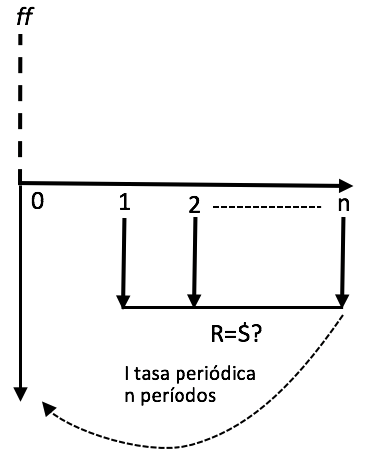
\includegraphics[height=6cm]{4_8}
\end{center}

\begin{equation*}
	VP=(1+i)^{-1}+(1+i)^{-2}+...+(1+i)^{-n} \hspace{35} \textit{Valor presente} \\
\end{equation*}

Para simplificar esta ecuación, podría seguirse un procedimiento similar al realizado para el valor final; sin embargo el camino más corto consiste en reemplazar el valor final.
\\\\
$VP=VF(1+i)^{-n}$ \hspace{35} \textit{Valor presente} \\


Si $VF$ lo reemplazamos por su equivalente se tiene:

\begin{equation*}
	VP = \frac{(1+i)^{n-1}}{i} (1+i)^{-n} = \frac{(1+i)^{n-1}}{i}\\
\end{equation*}

De donde se concluye que:

\begin{equation*}
	VP = \frac{1-(1+i)^{-n}}{i}
\end{equation*}

Las fórmulas anteriores fueron deducidas para una renta de \$1 pero si la renta hubiese sido de \$R, el valor final VF o el valor presente VP hubiese sido R veces mayor. Por tanto podemos escribir

\begin{align*}
	VP=R \frac{1-(1+i)^{-n}}{i}\hspace{35}\ Valor\ presente\ serie\ uniforme \ vencida
	\\\\
	VF=R \frac{(1+i)^{n}-1}{i}\ \hspace{35}\ Valor\ futuro\ serie\ uniforme\ vencida
\end{align*}
\\
\\\\
\textbf{Ejemplo 2}
\\

Un documento estipula pagos trimestrales de \$80.000, durante 6 años. Si este documento se cancela con un solo pago de:

\hspace{35} A. VP = \$?   al principio.

\hspace{35} B. VF = \$?   al final.
\\
con una tasa del 32\% nominal anual trimestre vencido.
\\\\
\textbf{Solución:}
\\

El número de pagos es $n=24\ ptv$,
\\
R = \$80.000 
\\

a. Diagrama de flujo: \\El diagrama representa el pago de una serie de \$80.000 en 24 períodos trimestrales vencidos, y de igual forma se observa el valor presente como pregunta del problema, de ¿Cuánto sería ese pago trasladando el pago final con todo y sus intereses a día de hoy (VP) ?       
\begin{center}
	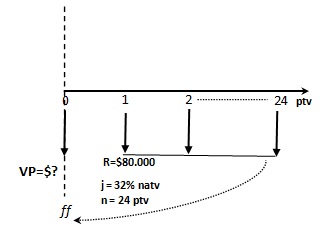
\includegraphics[height=5.7cm]{4_9}
\end{center}
b. Declaración de Variables:\\

	$R= \$80.000$
	\\
    VP = \$ ? \\
	$i=\frac{32\%natv}{4 ptv}=8\% \ ptv $\\
	n= 24 ptv\\
	
\clearpage
c. Declaración de Fórmulas:\\ 

$	VP=R\frac{1-(1+i)^{-n}}{i}$ \hspace{35 } \textit{\ Valor \ presente \ serie \ uniforme \ vencida}\\

d. Desarrollo Matemático:\\

$	VP=\$80.000 \frac{1-(1+0.08)^{-24 }}{0.08}=\$842.301$\hspace{35} \textit{Ecuación de valor}
\\

e. Respuesta:\\
El valor del único pago al inicio es de VP= \$842.301\\



\textbf{Segunda Parte}\\

a. Diagrama de Flujo:\\

Se calcula el pago total al final de los 24 períodos, para así proceder a calcular el pago presente o al día de hoy.

\begin{center}
	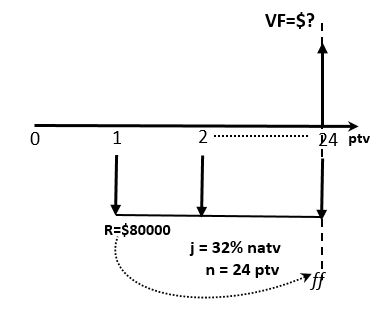
\includegraphics[height=5.4cm]{4_10}
\end{center}
b. Declaración de variables:\\

	$R= \$80.000$\\
	VF= \$ ? \\
	i=8\% ptv\\
	n= 24 ptv\\


c. Declaración de fórmulas:

\begin{equation*}
	VF=R \frac{(1+i)^{n}-1}{i} \\ Valor \ futuro \ serie \ uniforme \ vencida
\end{equation*}
d. Desarrollo matemático:
\begin{equation*}
	VF=\$80.000 \frac{(1+0.08)^{24}-1}{0.08}=\$5'341.181 \hspace{35}\textit{Ecuación de valor}
\end{equation*}

e. Respuesta:\\

El valor del único pago al final de la serie uniforme vencida es de VF=\$ 5'341.181\\

\clearpage

\textbf{Ejemplo 3}

\newline \vspace{1mm}

Una persona empieza el día primero de julio de 1986 a hacer depósitos de \$1.000 mensualmente el día primero de cada mes. Estos depósitos son efectuados en una entidad financiera que le paga el 24\% namv; pero a partir del primero de octubre de 1987 [15 períodos], decidió que de ahí en adelante sus depósitos serían de \$2.500. El último depósito lo hizo el primero de agosto de 1989. Si el primero de diciembre de 1989 decide cancelar la cuenta. ¿Cuál será el monto de sus ahorros?

\newline \vspace{2mm}

a. Diagrama de Flujo:

\newline \vspace{2mm}
Este diagrama de flujo representa dos series uniformes periódicas, una en la que el pago mensual es de \$1.000 y la otra en el que el pago mensual es de \$2.500, por ende se calcula un valor final de la primera serie uniforme y un valor final de la segunda serie uniforme, sumándole el valor final de la primera serie uniforme trasladando todos los períodos de la segunda serie uniforme.

\newline \vspace{2mm}

Para facilitar el cálculo del valor de los periodos se llenó la siguiente tabla:

\begin{tabular}
{ |p{1.3cm}|p{3.5cm}|p{3.5cm}|p{1.5cm}|p{1.5cm}|p{1.3cm}| }
\hline 
\rowcolor{white!50}              
\begin{center}\textbf{Periodo\\ (1)} \end{center} & \begin{center} \textbf{Número de meses desde el inicio del año inicial hasta la fecha inicial\\ (2)} \end{center} & \begin{center} \textbf{Número de meses desde el inicio del año final hasta la fecha final\\ (3)} \end{center} & \begin{center} \textbf{Año de la fecha inicial\\ (4)} \end{center} & \begin{center} \textbf{Año de la fecha final\\ (5)} \end{center} & \begin{center} \textbf{Valor\\ (6)} \end{center}\\ \hline

n$_{1}$ & 6 pmv & 9 pmv   & 1986 pav & 1987 pav & 15 pmv\\ \hline
n$_{2}$ & 9 pmv & 8 pmv   & 1987 pav & 1989 pav & 23 pmv\\ \hline
n$_{3}$ & 9 pmv & 12 pmv  & 1987 pav & 1989 pav & 27 pmv\\ \hline
n$_{4}$ & 8 pmv & 12 pmv  & 1989 pav & 1989 pav & 4 pmv\\ \hline

\end{tabular}\\

\newline \vspace{2mm}

El cálculo del valor de la columna 6 se llevó a cabo a través de la siguiente ecuación:

\newline \vspace{2mm}

\\$(6)=\big\{{\frac{12pmv}{1pav}[(5)-(4)]+(3)\big\}-(2)$ \hspace{35 pt} \textit{Cálculo de períodos mensuales vencidos}\\

\begin{center}
	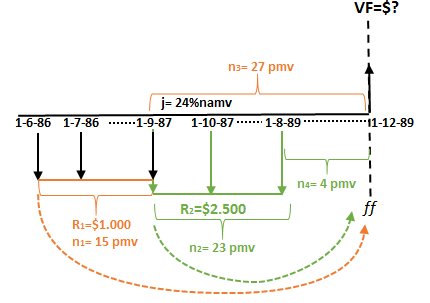
\includegraphics[height=9cm]{4_11}
\end{center}


b. Declaración de variables\\\\
%\begin{center}
    $VF$= \$?\\
	j=24\% namv\\
	$i=\frac{24\% namv}{12 pmv} = 2\%$ pmv\\
	
    \begin{tabular}{ c p }
     \multirow{2}{4em}{$R_{1}$=\$1.000} & $n_{1}$ = 15 pmv \\ 
     & $n_{2}$ = 27 pmv \\ 
     \multirow{2}{4em}{$R_{3}$=\$2.500} & $n_{3}$ = 23 pmv \\
     & $n_{4}$ = 4 pmv \\    
    \end{tabular}
    
\vspace{5mm}

\\
c. Declaración de fórmulas:\\

	\\VF=R $\frac{(1+i)^{n}-1}{i}$ \hspace{35 pt} \textit{Valor futuro de serie uniforme vencida}\\

	F=P(1+i)^{n}  \hspace{60 pt} \textit{Valor futuro}
\vspace{5mm}

Observemos que hay 2 series periódicas: el depósito de \$1.000 y el despósito de \$2.500. La primera serie uniforme empieza el 1-6-86 (primero de junio de 1986) y termina el 1-9-87 (primero de septiembre de 1987) y la segunda serie uniforme empieza el 1-9-87 y termina el 1-8-89. De ésta forma la primera serie uniforme tendrá 15 períodos y su valor final deberá ser trasladado por 27 períodos para llevarlo a la fecha focal (desde el 1-9-87 hasta el 1-12-89). La segunda serie uniforme tendrá 23 períodos (tomamos en cuenta el punto cero de esta serie uniforme el 1-9-87) y su valor final lo debemos trasladar por 4 períodos y así la ecuación de valor será:
\\\\
d. Desarrollo matemático
\\
\begin{equation*}
	VF = \$1.000\frac{(1+0.02)^{15}-1}{0.02}*[1+0.02]^{27} + \$2500\frac{(1+0.02)^{23}-1}{0.02}*(1+0.02)^{4} \hspace{5}\textit{Ecuación de valor}
\end{equation*}
Donde se obtiene: \ $VF=\$ 107.574,69$
\\\\
\textit{NOTA: }Al cambiar de posición la fecha focal por ejemplo, si en lugar de ponerla al final se hubiera puesto al principio la respuesta no varía, aunque a primera vista la ecuación de valor es muy distinta.
\\\\
\textbf{Ejemplo 4}\\\\

Una deuda de \$50.000 se va a cancelar mediante 12 pagos periódicos mes vencidos de valor R. Con una tasa del 2\% periódica mes vencido, hallar el valor de la cuota mensual R situando:
\vspace{5mm}

 \hspace{35} A. La fecha focal el día de hoy.

 \hspace{35} B. La fecha focal en 12 meses.
 
\vspace{5mm}

Solución:
\\\\
A. La fecha focal el día de hoy.\\\\
En este caso usaremos la fórmula VP dada una serie uniforme vencida porque todo el flujo de caja debe ser trasladado al principio que es donde está la fecha focal y la ecuación de valor quedará así:
\\\\
a. Diagrama de flujo:\\

Se tiene un diagrama de flujo en el cual se contrajo una deuda de \$50.000 y se pagara con cuotas de R durante doce meses, calcular \$R si se tiene un interés de 2\% periódico mensual vencido.
\begin{center}
	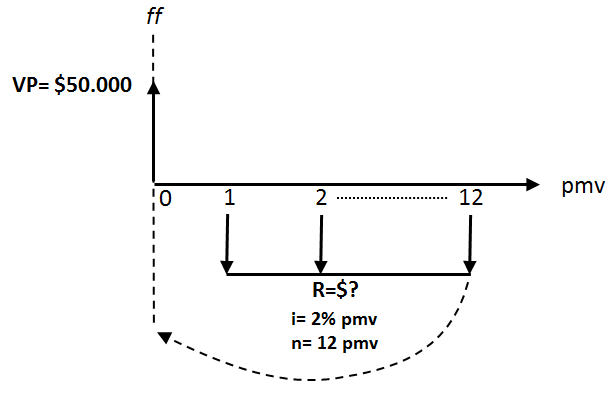
\includegraphics[height=6.5cm]{4_12}
\end{center}

b. Declaración de variables:\\

	VP=\$50.000
	\\
	i=2\% \ \ pmv\\
	n=12\ pmv
	\\
	R=\$?
	\\
c. Declaración de fórmulas:\\

	$VP=R [\frac{1-(1+i)^{-n}}{i}]$  \hspace{35}\textit{Valor presente  serie  uniforme vencida}\\
    \\

d. Desarrollo matemático:\\

	$\$50.000=R[\frac{1-(1+0.02)^{-12}}{0,02}] $ \hspace{35}\textit{Ecuación de valor}
	\\\\
$	R=\$4.727,98$\\

e. Respuesta:\\

El valor de la cuota mensual es de R=\$4.727,98. \\


B. Poniendo la fecha focal en 12 meses.\\

a. Diagrama de Flujo:\\
En este caso se calcula R con base a a la deuda de los \$50.000 trasladada doce meses al futuro.
\begin{center}
	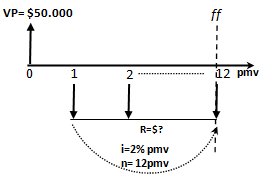
\includegraphics[height=5.5cm]{4_13}
\end{center}

b. Declaración de variables:

	P=\$50.000
	\\
	i=2\% \ \ pmv\\
	n=12\ pmv
	\\
	R=\$?
	\\

c. Declaración de fórmulas:


	\\\\
	VF=R$\frac{(1+i)^{n}-1}{i}$ \hspace{35}\textit{ \ \ Valor \ \ futuro \ \ serie \ \ uniforme \ \ vencida} \\
	
	F=P(1+i)^{n} \hspace{55}\textit{ \ \ Valor \ \ futuro \\}\\


Se utilizan las dos fórmulas porque todo el flujo de caja debe ser trasladado al punto 12 que es donde está la fecha focal, pero la deuda de los \$50.000 sigue en 0 lo cual implica que deberá ser trasladada a valor final junto con todos los pagos, entonces la ecuación quedará así:
\\\\
d. Desarrollo matemático:\\

	\$ 50.000 [1+0.02]^{12}=R [\frac{(1+0.02)^{12}-1}{0.02}] \hspace{35}\textit{Ecuación de valor}
	\\
	R=\$4.727,98\\

e. Respuesta:\\

El valor de la cuota mensual es de R=\$4.727,98.

\section{Series periódicas anticipadas (VP, VF, R, i, n)}

Una serie uniforme anticipada es aquella en que los pagos se hacen al principio del período. El valor presente y el valor final se representarán respectivamente por: VP$_{a}$ y VF$_{a}$.\\


	$VF_{a}=R \frac{(1+i)^{n}-1}{i}(1+i) $ \hspace{35}\textit{ Valor  futuro  serie  uniforme  anticipada}
	\\
	$VP_{a}=R \frac{1-(1+i)^{(-n)}}{i}(1+i)$
	\hspace{30}\textit{Valor  presente  serie  uniforme  anticipada}\\

\clearpage

Existen relaciones entre las series periódicas ordinarias y las series periódicas anticipadas, las cuales podrán ser deducidas del análisis de las series uniformes vencidas: a) Para facilitar el planteamiento de la ecuación de valor comenzamos con el flujo que está en n, siguiendo con el que está en n-1 y así sucesivamente hasta llegar al pago situado en 1, entonces para valor final con serie uniforme ordinaria la ecuación de valor quedará así:

\vspace{5mm}

      	$VF$_{a}$=1+ (1+i) +(1+i)^{2}+...+(1+i)^{n} $ \\
      	
\vspace{5mm}
\\
\textbf{Serie uniforme ordinaria:}
\begin{center}
    
	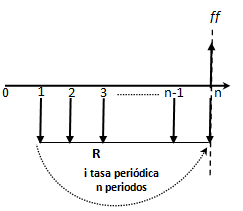
\includegraphics[height=5.1cm]{4_14}
	
\end{center}

Para la serie uniforme anticipada en valor final, la gráfica del flujo de caja quedará así:
\textbf{\\ \\ Serie uniforme anticipada:} 
\begin{center}
    
	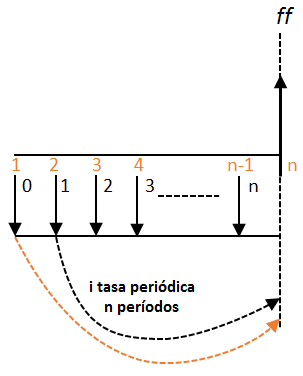
\includegraphics[height=6cm]{4_15}
	
\end{center}
Observe que en este caso se ha usado una doble numeración la que está encima de la línea de tiempo indica el número del pago, mientras que la que se encuentra debajo de la línea de tiempo señala los períodos. \\

En el período 0 que es el comienzo del primer período se está haciendo el pago número 1, en el período 1 que es el final del primer período pero a su vez es el comienzo del segundo período y por eso se realiza el segundo pago y así sucesivamente hasta que lleguemos al punto n-1. La ecuación de valor para la anterior situación será:
\vspace{5mm}
    	$VF$_{a}$=(1+i)^{1}  +(1+i)^{2}+...+(1+i)^{n-1}+(1+i)^{n}$
\vspace{5mm}

\clearpage

La diferencia entre las dos series periódicas consiste en que la serie de la serie uniforme ordinaria empieza con 1 y termina con $(1+i)^{(n-1)}$, en cambio, la serie de la serie uniforme anticipada comienza con $(1+i)$  y termina con $(1+i)^{n}$. Si a la serie anticipada se le agrega un 1 y se le resta al final y, si además, le introducimos el paréntesis angular, el resultado no se altera.

\vspace{5mm}
        $VFa=[1+(1+i) +(1+i)^{2}+(1+i)^{3}...+(1+i)^{(n-1)} ]+(1+i)^{n-1}$
\vspace{5mm}

Obsérvese que la parte que está dentro del paréntesis es igual a la serie ordinaria, por tanto, podemos decir que:

\vspace{5mm}
        $VFa=VF+(1+i)^{n}-1$
\vspace{5mm}

Si reemplazamos VF por su equivalente $\frac{(1+i)^{n}-1}{i}$ se tendrá:

\vspace{5mm}
	VF$_{a}$=$\frac{(1+i)^{n}-1}{i}$+$i\frac{(1+i)^{n}-1}{i}$
\vspace{5mm}

Si se factoriza  $\frac{(1+i)^{n}-1}{i}$, se tendrá:

\vspace{5mm}
    VF$_{a}$=$\frac{(1+i)^{n}-1}{i}$(1+i) \ \  Pero \ \ como \ \ $VF = \frac{(1+i)^{n}-1}{i}$
\vspace{5mm}

Entonces se tiene que:

\vspace{5mm}
	$VF_{a} = VF$_{a}$=$\frac{(1+i)^{n}-1}{i}$(1+i) = VF (1+i)$  \hspace{35}\textit{ Valor  futuro  serie  uniforme  anticipada}

\vspace{5mm}

\textbf{Ejemplo 5}

\vspace{5mm}

Una persona arrienda una casa en \$50.000 pagaderos por mes anticipado, Si tan pronto como recibe cada arriendo, lo invierte en un fondo que le paga el 2\% periódico mes vencido ¿Cuál será el monto de sus ahorros al final de un año? 
\\\\
a.Diagrama de flujo:\\

\begin{center}
	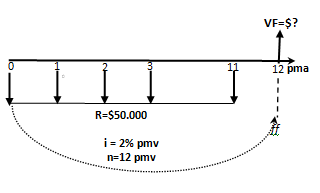
\includegraphics[height=5.1cm]{4_16}
\end{center}

\clearpage

b. Declaración de variables: \\

	R=\$50.000  \\ 
	i=2\%  pmv \\
	n=12  pmv\\
	VF=\$?\\


c. Declaración de fórmulas:\\

	VF$_{a}$=R $\frac{(1+i)^{n}-1}{i}$(1+i)  \hspace{35}\textit{Valor futuro serie  uniforme anticipada}\\
\\\\
d. Desarrollo matemático:\\


	$VF_{a}=\$50.000 \frac{(1+0.02)^{12}-1}{0.02}(1+0.02)$ \hspace{35}\textit{Ecuación de valor}
	\\\\
	$VF_{a}=\$684.016,58$ \\
	
e. Respuesta:\\

El monto final de los ahorros sera de \$684.016,58 \\

\section{Series periódicas ordinarias en valor presente (VP, VF, R, i, n)}
La ecuación de valor la comenzamos a plantear con el pago que está en 1 y terminando con el pago que esté en \textbf{n}.

\begin{center}
	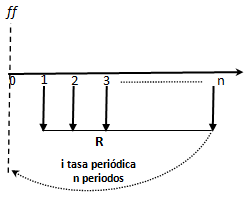
\includegraphics[height=5cm]{4_17}
\end{center}


	VP= (1+i)^{-1}+(1+i)^{-2}+(1+i)^{-3}+...+(1+i)^{-(n-1)}+(1+i)^{-n}

\clearpage

\section{Series periódicas anticipadas en valor presente}

La diferencia entre las dos series estriba en que la ordinaria empieza con $1$ y termina con $(1+i)^{-n}$ y la anticipada comienza con $1$ y termina con $(1+i)^{-(n-1)}$.

\begin{center}
	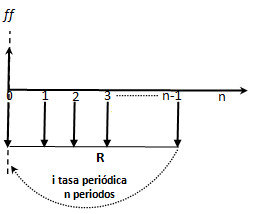
\includegraphics[height=5.6cm]{4_18}
\end{center}

Y la correspondiente ecuación de valor quedará así:\\
\begin{center} 

	$VP_{a}=1+[(1+i)^{-1}+(1+i)^{-2}+...+(1+i)^{-(n-1)} ] -(1+i)^{-n}$
	
\end{center}

Si a la serie de la serie uniforme anticipada le agregamos $(1+i)^{-n}$ y le restamos esa misma cantidad y además le introducimos un paréntesis angular, el resultado no se altera entonces:

\vspace{5mm}

	$VP_{a}= 1+[(1+i)^{-1} +(1+i)^{-2}+...+(1+i)^{-(n-1)} +(1+i)^{-n} ] -(1+i)^{-n}$
	
\vspace{5mm}
Ahora podemos observar que la serie que está dentro del paréntesis angular corresponde a la serie ordinaria, por tanto podemos decir que:

\vspace{5mm}
    
$VP_{a}= 1+VP-(1+i)^{-n}=VP+1-(1+i)^{-n}$
\vspace{5mm}

Si los dos últimos términos de la ecuación anterior se encierran en un paréntesis angular y se multiplican y dividiendo por i, no se altera la igualdad, por tanto se tiene:

\vspace{5mm}
	$VP_{a}=VP+\frac{i (1-i)^{-n} }{i}=VP+iVP$
\vspace{5mm}

Factorizando VP se tiene la fórmula final

\vspace{5mm}
	$VP_{a}=VP$ $\frac{1-(1+i)ˆ{-n}}{i}$(1+i) \hspace{35}\textit{Valor presente de una serie uniforme anticipada}\\
\vspace{5mm}

\textbf{Ejemplo 6}

\vspace{5mm}

El contrato de arriendo de una casa estipula pagos mensuales de \$40.000, al principio de cada mes durante un año. Si suponemos un interés del 30\% nama. ¿Cuál será el valor del pago único que, hecho al principio del contrato, lo cancelaría en su totalidad?
\\\\
\clearpage

\textbf{Solución}
\\
a. Diagrama de Flujo:\\

\begin{center}
	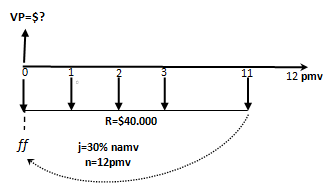
\includegraphics[height=5.3cm]{4_19}
\end{center}
b. Declaración de variables: \\

	R=\$40.000 \\
	VP_{a}=\$?\\
	j=30\% nama \\
	i= \frac{30\%nama}{12 pma} =2,5\% pma\\
	n=12pma\\

c. Declaración de fórmulas:\\

	$VP_{a}=R$ $\frac{1-(1+i)^{-n}}{i}$ $(1+i)$  \hspace{35} \textit{Valor presente serie uniforme anticipada}\\


d. Desarrollo matemático:\\

	VP$_{a}$=\$40.000 $\frac{1-(1+0.025)^{-12}}{0,025}$  $(1+0.025)$ \hspace{35}\textit{Ecuación de valor}\\
	VP$_{a}$=\$420.528,34\\
	
e. Respuesta:\\

El valor del pago sera de $\$420.528,34$\\


\section{Otro enfoque de las series periódicas anticipadas}
Podemos calcular el valor presente de la serie uniforme anticipada como si fuera una serie uniforme vencida, de la siguiente manera, si retiramos el pago que está en 0 y también retiramos el período que se inicia en 11 y termina en 12, nos queda una serie ordinaria de 11 pagos con 11 períodos, luego forma una serie uniforme vencida porque empieza en período y termina con pago, el pago que está en cero se puede considerar como un pago adicional que no pertenece a la serie uniforme, tal como se aprecia en la gráfica anterior.\\

Este enfoque es el más utilizado al resolver ejercicios de series periódicas anticipadas. 
\\\\
a. Diagrama de flujo:\\

El siguiente diagrama representa un traslado de períodos anticipados a períodos vencidos, sin afectar la serie.
\begin{center}
	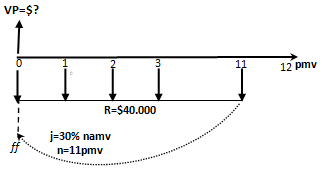
\includegraphics[height=5cm]{4_20}
\end{center}

b. Declaración de variables:\\

$	
	R=\$40.000\\	
	P_{0}=\$40.000\\
	i=2,5\% pmv \\
    n={11}\ pmv\\
	n_{0}=12 pmv\\
$

c. Declaración de fórmulas:\\

	VP=R$\frac{(1-(1+i)^{-n})}{i}$ \hspace{35}\textit{Valor  presente de  una  serie  periódica  vencida}\\


d. Desarrollo matemático: \\                                

	VP_{11}=\$40.000 \frac{1-(1+0,025)^{-11}}{0,025}\\
	VP_{11}=\$380.568,35\\
	VP=VP_{11}+P_{0}\\
	VP=\$380.568,35+\$40.000\\
	VP=\$420.568,35\\\\


\textbf{Ejemplo 7}

\vspace{5mm}
Una persona necesita tener reunidos \$100.000 para el día 15-10-95, para tal fin constituye un fondo mediante depósitos trimestrales de R efectuándose el primero el día 15-7-90 y el último el 15-4-95 además se efectuará un depósito extraordinario de \$8.000 el 15-1-93. Si el fondo paga el 24\% nominal anual trimestre vencido. ¿Cuál es el valor de R? Considerar un año de 360 días.
\\\\
\textbf{Solución:}
\\
a. Diagrama de Flujo:\\

Este diagrama representa los pagos Trimestrales de \$R mas un pago extraordinario de \$8000. Calcular \$R de tal forma que al final tenga reunido \$100.000

\vspace{5mm}

De 15-04-1990 al 15-04-1995 hay 5 pav equivalente a 20 ptv. El VF se debe trasladar  de 15-04-1995 a 15-10-1995, esto es 6 meses equivalentes a 2 ptv, mediante la fórmula $F = P (1+i)^n.$

\vspace{5mm}

El valor P_{3}= $$\$8.000$ se debe trasladar del 15-01-1993 al 15-10-1995, esto es a 33 meses después, equivalentes a 11 ptv.

\begin{center}
	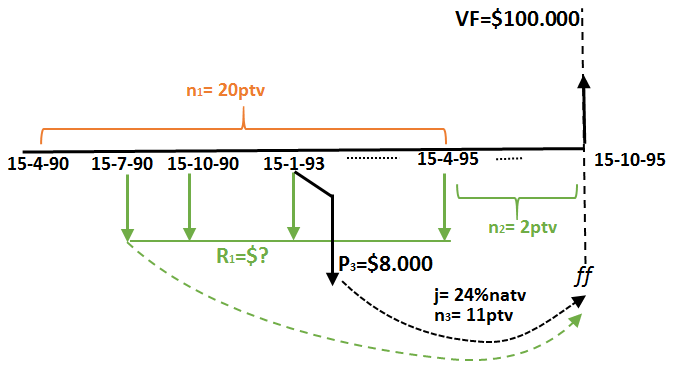
\includegraphics[height=6cm]{4_21}
\end{center}

b. Declaración de variables:\\

	VF=\$100.000\\
	$R_{1}=\$?$\\
	P_{3}=\$8.000 \\
	$j=24\% natv$\\
	$i= $\frac{24\%natv}{4ptv}$ $= 6\% ptv \\
	$n_{1}=20$ ptv\\
	$n_{2}=2 $ ptv \\
	$n_{3}=11 $ ptv \\

c. Declaración de fórmulas:\\

	VF = R $\frac{((1+i)^{n}-1)}{i} $ \hspace{35}\textit{ Valor futuro serie uniforme vencida}\\\\
	F = P(1+i)^{n}  \hspace{67}\textit{Valor futuro}

d. Desarrollo matemático:\\

	R_{1}(\frac{((1+0,06)^{20}-1)}{0,06})*(1+0,06)^{2}+\$8.000 (1+0,06)^{11}=\$100.000 \hspace{35}\textit{Ecuación de valor}\\
	R_{1}(\frac{((1,06)^{20}-1)}{0,06})*(1,06)^{2}+\$8.000 (1,06)^{11}=\$100.000\\\\
	$R_{1}=\$2.051,99$\\
	
e. Respuesta:

El valor de R es \$2.051,99

\section{Tabla de amortización}
La amortización consiste en pagar una deuda, mediante una serie de pagos; el comportamiento de la deuda y los intereses se pueden mostrar en una tabla denominada tabla de amortización.\\
Una tabla de amortización debe tener como mínimo, cinco columnas: la primera muestra el número del período, la segunda nos muestra el saldo de la deuda, es decir, el capital insoluto a medida que van pasando los períodos, la tercera nos muestra los intereses que se van causando período a período, la cuarta columna nos muestra la cuota o cantidad que se paga en cada período y la quinta columna nos muestra la porción de la cuota que se usa para disminuir la deuda, es decir, la cantidad que se amortiza, también se le denomina abono a capital.
\vspace{1mm}

Haciendo uso del ejemplo 9 explicaremos la forma de construir una tabla de amortización.\\

\textbf{Ejemplo 9}

\vspace{5mm}

Elaborar una tabla para amortizar la suma de \$10.000 en 4 pagos iguales, suponiendo una tasa de interés de 40\% nominal anual trimestre vencido.
\\\\
\textbf{Solución:}
\\
Primero elaboramos una gráfica del flujo de caja y calculamos el valor de la cuota.
\\

\vspace{5mm}

a. Diagrama de Flujo: \\

El diagrama representa la salida de capital de \$10.000 y como se amortizaría en pagos iguales en cuatro períodos, con un interés del 40\%natv.

\begin{center}
	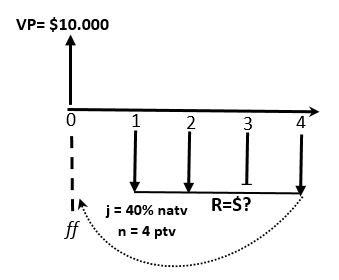
\includegraphics[height=6cm]{4_22}\\
\end{center}

Se establece como fecha local el período 0.
Una tabla de amortización muestra período a período, la forma como se va cancelando una deuda inicial. Para construir la tabla de amortización, primero se calcula la cuota de la serie uniforme vencida. Luego se registra la cuota en la columna tercera de la tabla de cinco columnas, compuesta por las columnas de: período, deuda  insoluta, Intereses, cuota o pago y  amortización. La ultima fila de la columna capital insoluta debe ser igual a 0.

\vspace{5mm}

b. Declaración de variables:

\vspace{5mm}

De lo anterior deducimos que las variables son:\\

	j=40\% \ \ natv \\ 
	i=10\% \ \ ptv\\
	n=4 \ \ ptv \\
	VP = \$10.000

\vspace{5mm}

c. Declaración de fórmulas:

\vspace{5mm}

	VP=R$\frac{(1-(1+i)^{-n})}{i}$ \hspace{35}\textit{Valor presente serie uniforme vencida}

\vspace{5mm}

d. Desarrollo Matemático\\


$	\$10.000=R\frac{(1-(1+0,1)^{-4})}{0,1}$\hspace{35}\textit{Ecuación de valor}\\ \\
	R=\$ 3.154,70\\

e. Respuesta:

Los pagos quedarán organizados de la siguiente manera:
\vspace{5mm}

\begin{center}
\begin{tabular}{ |p{1.5cm}|p{3cm}|p{2cm}|p{2cm}|p{3cm}| }
\hline 
\rowcolor{white!50}              %
\begin{center}\textbf{Periodo\\ (1)} \end{center} & \begin{center} \textbf{Capital Insoluto\\ (2)=P-(5)}\end{center} & \begin{center} \textbf{Intereses\\ (3)=Pi} \end{center} & \begin{center} \textbf{Pago\\ (R)} \end{center} & \begin{center} \textbf{Amortización\\ (5)=R-(3)} \end{center}\\ \hline

0 & \$ 10.000,00   & \$ -      & \$ -      & \$ - \\ \hline 

1 & \$ 7.845,30    & \$ 1.000,00  & \$ 3.154,70  & \$ 2.154,70 \\ \hline 

2 & \$ 5.475,13    & \$ 784,53    & \$ 3.154,70  & \$ 2.370,17 \\ \hline 

3 & \$ 2.867,94    & \$ 547,51    & \$ 3.154,70  & \$ 2.607,19 \\ \hline 

4 & \$ 0,03        & \$ 286,79    & \$ 3.154,70  & \$ 2.867,91 \\ \hline 

\end{tabular}
\end{center}

\section{Tabla de capitalización}
La palabra capitalización tiene otros significados afines, en este libro por capitalización entenderemos el reunir un capital mediante depósitos periódicos.
\\\\
Una tabla de capitalización nos muestra, período a período, la forma como se va reuniendo un capital, su conformación es similar a la de amortización y básicamente debe tener 5 columnas que en su orden las denominaremos: período, capital reunido o monto, intereses, depósito o cuota y la última columna que se denomina capitalización o incremento por período.
\\\\
La explicación de la forma de elaborar una tabla de capitalización la daremos con el siguiente ejemplo:
\\\\
\textbf{Ejemplo 10}

\vspace{5mm}

Elaborar una tabla para capitalizar la suma de \$300.000 en 15 meses, haciendo depósitos trimestrales iguales en un fondo que paga una tasa del 32\% nominal anual trimestre vencido.
\\\\
\textbf{Solución:}
\\
a. Diagrama de Flujo:\\

El diagrama representa los pagos R durante 5 períodos trimestrales a los cuales se le abona un 8\%ptv para obtener un valor final de \$300.000.

\begin{center}
	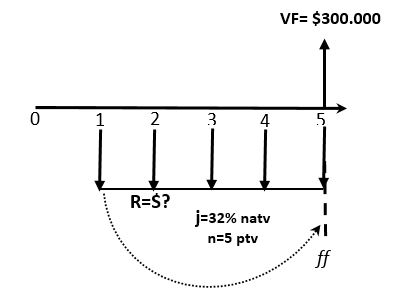
\includegraphics[height=6cm]{4_24}\\
\end{center}

b. Declaración de variables:\\

	j=32\% natv  \\
	i=8\% ptv \\
	n=5 ptv \\
	VF=\$300,00 \\
	R=\$? \\
	
\vspace{5mm}

c. Declaración de fórmulas:

\vspace{5mm}
	VF=R$\frac{((1+i)^{n}-1)}{i}$ \hspace{35}\textit{Valor futuro serie uniforme vencida}
\vspace{5mm}

d. Desarrollo matemático:\\
\\
Ahora procederemos a plantear la ecuación de valor y calcular la cuota.\\

$	\$300.000=R\frac{((1+0,08)^{5}-1)}{0,08}$ \hspace{35}\textit{Ecuación de valor}\\
	R=  \$51.136,94 \\ \\

Los pagos quedaran organizados de la siguiente manera:\\

e. Respuesta:

\begin{center}
\begin{tabular}{ |p{1.5cm}|p{3cm}|p{2cm}|p{2cm}|p{3cm}| }
\hline 
\rowcolor{white!50}              %
\begin{center}\textbf{Periodo\\ (1)} \end{center} & \begin{center} \textbf{Acumulado\\ (2)=P+(5)}\end{center} & \begin{center} \textbf{Intereses\\ (3)=Pi} \end{center} & \begin{center} \textbf{Depósito\\ (R)} \end{center} & \begin{center} \textbf{Capitalización\\ (5)=(3)+(4)} \end{center}\\ \hline

0 & \$ 51.136,94    & \$ 0,00       & \$ 51.136,94      & \$ 51.136,94 \\ \hline 

1 & \$ 106.364,84   & \$ 4.090,96   & \$ 51.136,94  & \$ 55.227,90 \\ \hline 

2 & \$ 166.010,97   & \$ 8.509,19   & \$ 51.136,94  & \$ 59.646,13 \\ \hline 

3 & \$ 230.428,79   & \$ 13.280,88  & \$ 51.136,94  & \$ 64.417,82 \\ \hline 

4 & \$ 300.000,00   & \$ 18.434,27  & \$ 51.136,94  & \$ 69.571,21 \\ \hline 

\end{tabular}
\end{center}

\clearpage

\textbf{Ejemplo 11}

\vspace{5mm}

Calcular la tasa a la cual una deuda adquirida de \$80.000 se cancela mediante el pago de doce cuotas mensuales de \$11.000.
\\\\
\textbf{Solución:}
\\
a. Diagrama de flujo:\\

El diagrama representa la cancelación de una deuda adquirida de de dinero de \$80.000, y se cancela en doce pagos mensuales R= \$11.000 se debe calcular i\% ? periódico mes vencido para cancelar los \$80.000

\begin{center}
	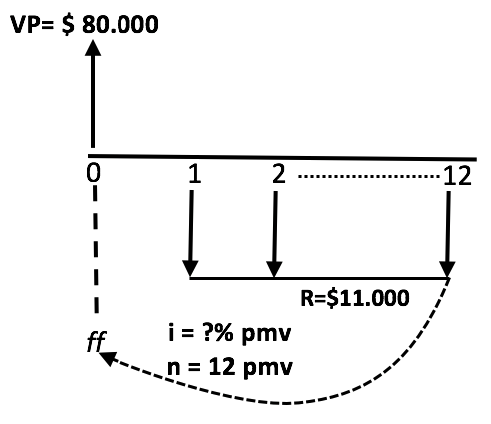
\includegraphics[height=6cm]{4_26}
\end{center}

Se establece como fecha focal en el período 0.
Se construye el diagrama de flujo con una serie uniforme vencida negativas.\\

b. Declaración de variables:

\vspace{5mm}
	VP=\$80.000\\
	i=?\% pmv\\
	n=12 \ \ pmv \\
	R=\$11.000
\vspace{5mm}

c. Declaración de fórmulas:

\vspace{5mm}
	VP=R$\frac{1-(1+i)^{-n}}{i}$  \hspace{35}\textit{Valor presente serie uniforme vencida}
\vspace{5mm}

La solución al problema consiste en hallar la tasa i=?\% pmv a la cual la igualdad es cierta, para ello, podemos resolver el problema manualmente usando la interpolación, vista en el capítulo anterior, para lo cual igualamos la ecuación a cero y hallamos dos valores de i=?\% pmv tal que la función sea una vez positiva y otra vez negativa así:
\\

d. Desarrollo matemático

\vspace{5mm}
	\$80.000-\$11.000$\frac{1-(1+i)^{-12}}{i}=0$ \hspace{35}\textit{Ecuación de valor}
\vspace{5mm}

\clearpage

Buscando el valor correspondiente al 8\% y al 9 \% se tiene
\begin{center}
	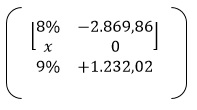
\includegraphics[height=2.5cm]{4_27}
\end{center}
Planteando las proporciones se tiene:\\

	$\frac{(8-9)}{(8-i)}=\frac{(-2.869,86-1.232,02)}{(-2.869.86-0)}=0 $\\

De donde se obtiene que i = 8.7\% pmv\\

e.Respuesta\\

La tasa sera de 8.7\% pmv\\

